\documentclass[../../main.tex]{subfiles}

\graphicspath{{images/Projektmanagement/}{../../images/Projektmanagement/}{include_pdf/}{../../include_pdf/}}

\begin{document}
\subsection{Projektmanagement}
Dieses Kaptitel beschreibt das Projektmanagement des Team 28. Es wird auf die Organisation im Team, die Aufteilung der Arbeitspakete und Zeitplanung eingegangen.

\subsubsection{Orgramigramm}
Die Abbildung \ref{fig:organigramm} zeigt die Organisation im Team auf. Das Team ist in die einzelnen Disziplinen Maschienentechnik, Elektrotechnik und Informatik aufgeteilt. Zusätzlich gibt es einen Projektleiter, dieser ist Verantwortlich für die Kommunikation mit den Fachdozenten und ist bei allfälligen Abwesenheiten von Teammitgliedern informiert.


\begin{figure}[H] \centering
    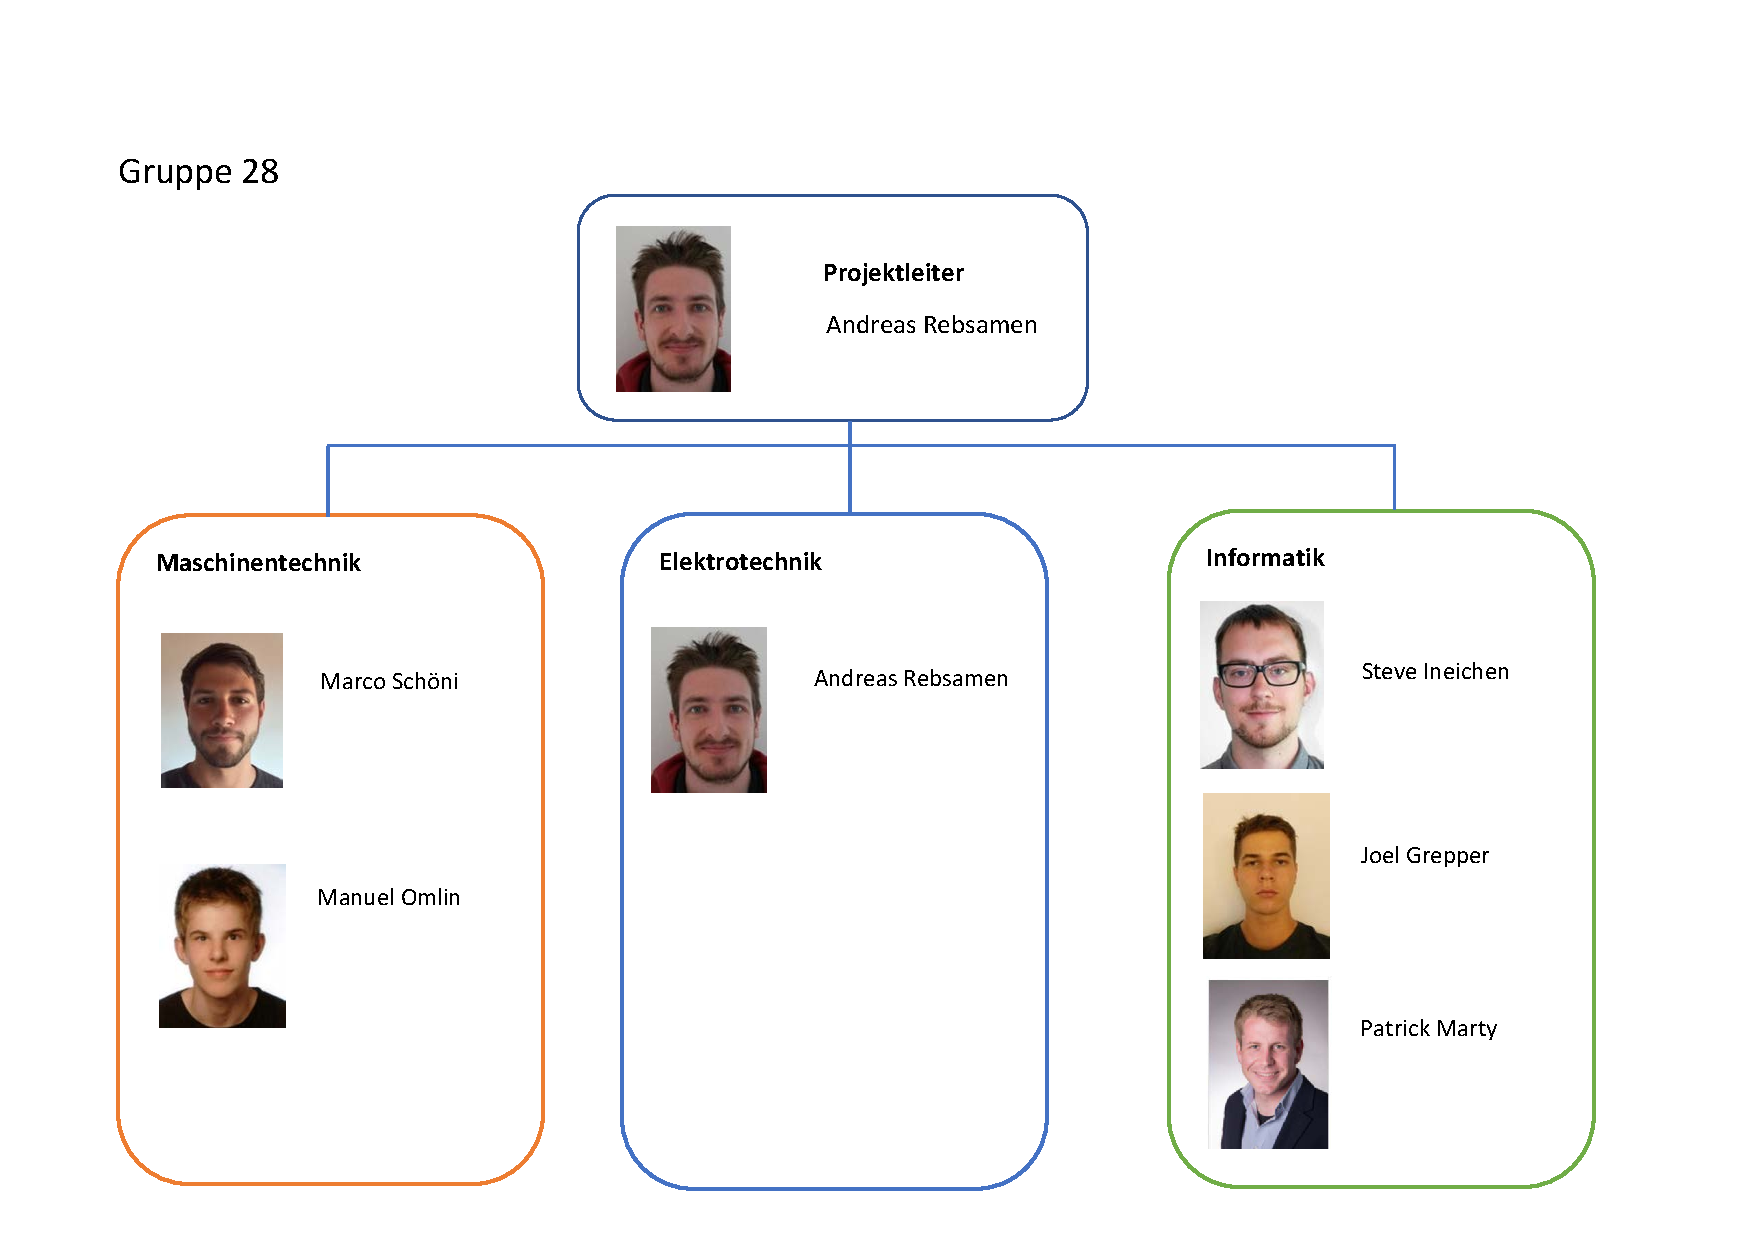
\includegraphics[page=1,width=.9\textwidth, trim=1cm .5cm 1cm 3.2cm, clip]{Organigramm.pdf}
    %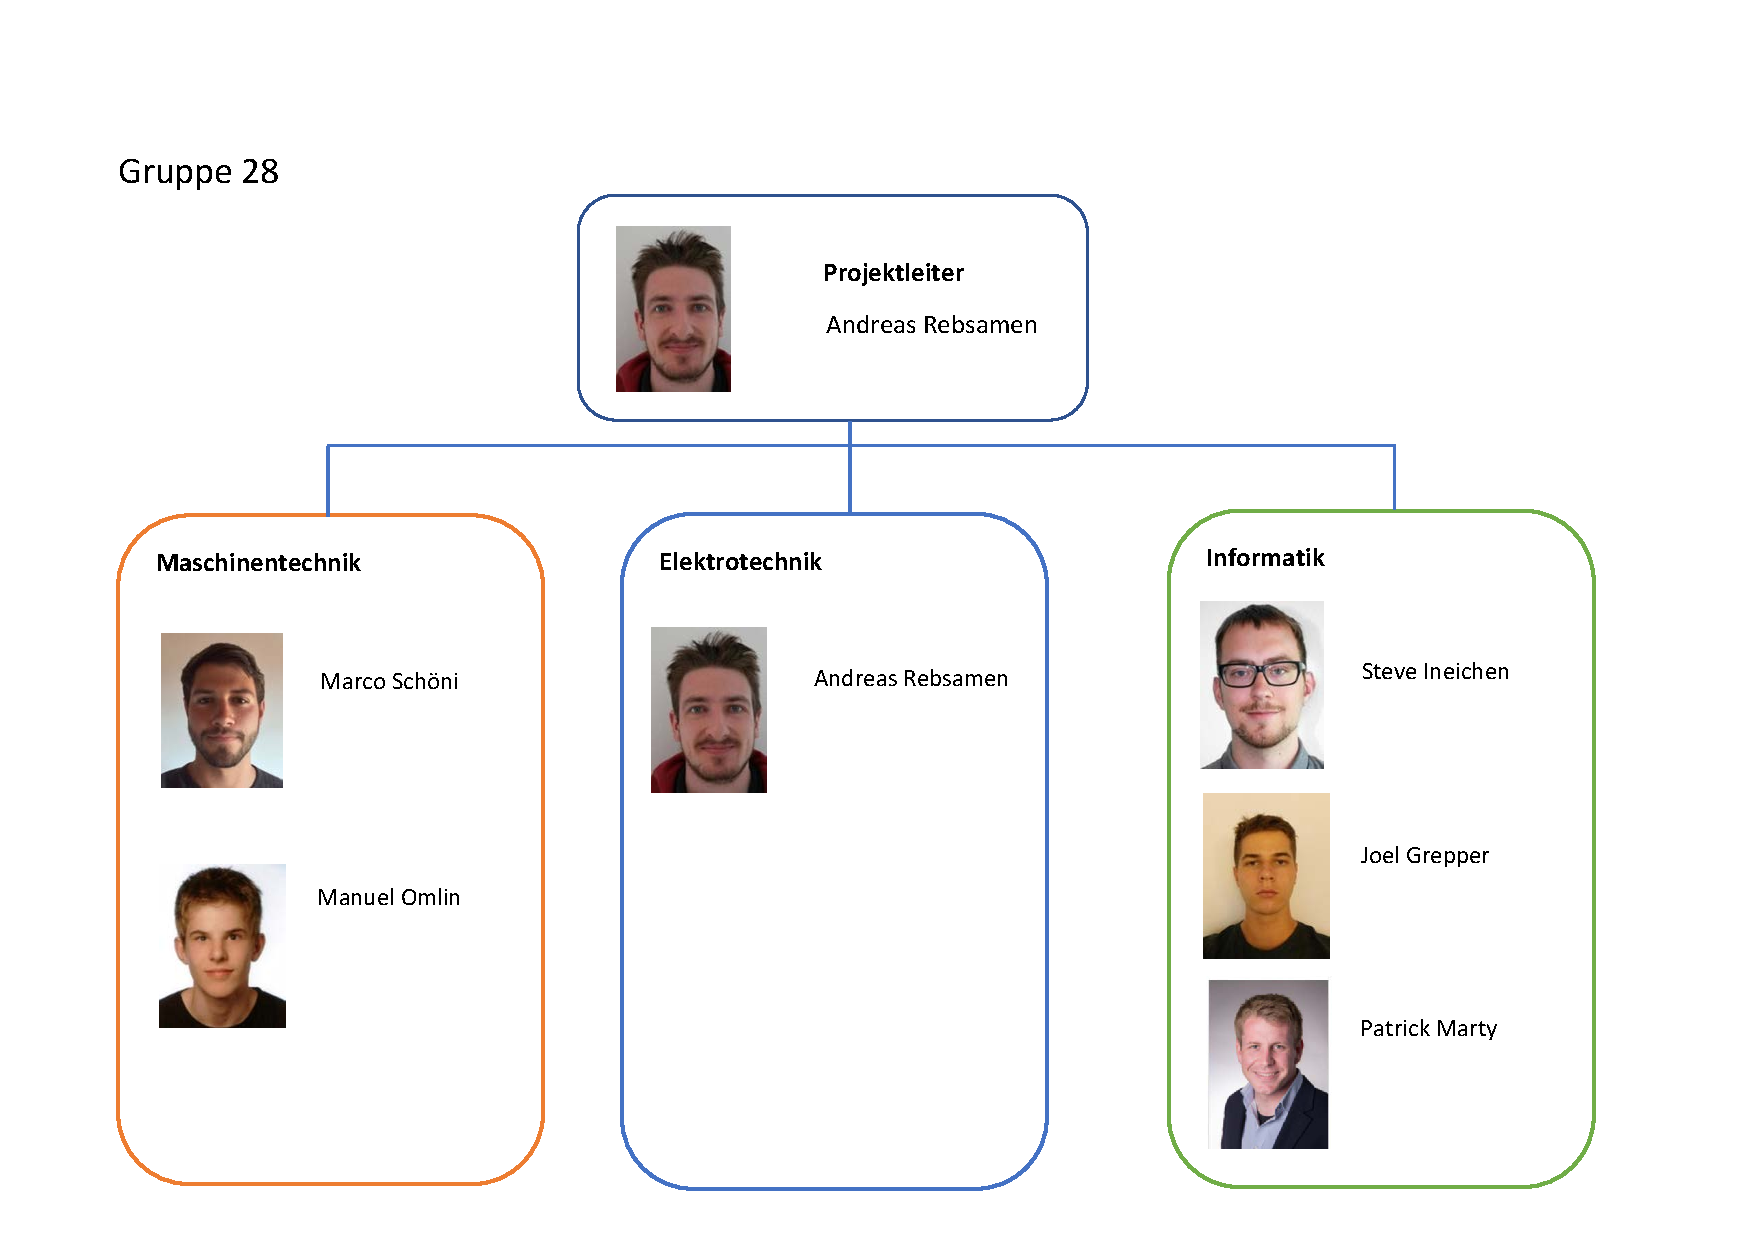
\includepdf[scale=0.8,clip,trim=20mm 7mm 20mm 32mm,pages=-,pagecommand={},nup=1x1, offset=0 -0cm]{Organigramm.pdf} 
    \caption{Organigramm Team 28}
    \label{fig:organigramm}
\end{figure}

\subsubsection{Zeitplanung}
Mit den groben Arbeitspaketen wurde eine Zeitorientierte Projektstruktur (Abbildung \ref{fig:projektplanung}) erstellt. In dieser ist festgehalten, welcher Person oder Disziplin ein Arbeitspaket zugeteilt ist, ob diese neu, in Abreit oder abgeschlossen ist. \\

\begin{figure}[H] \centering
    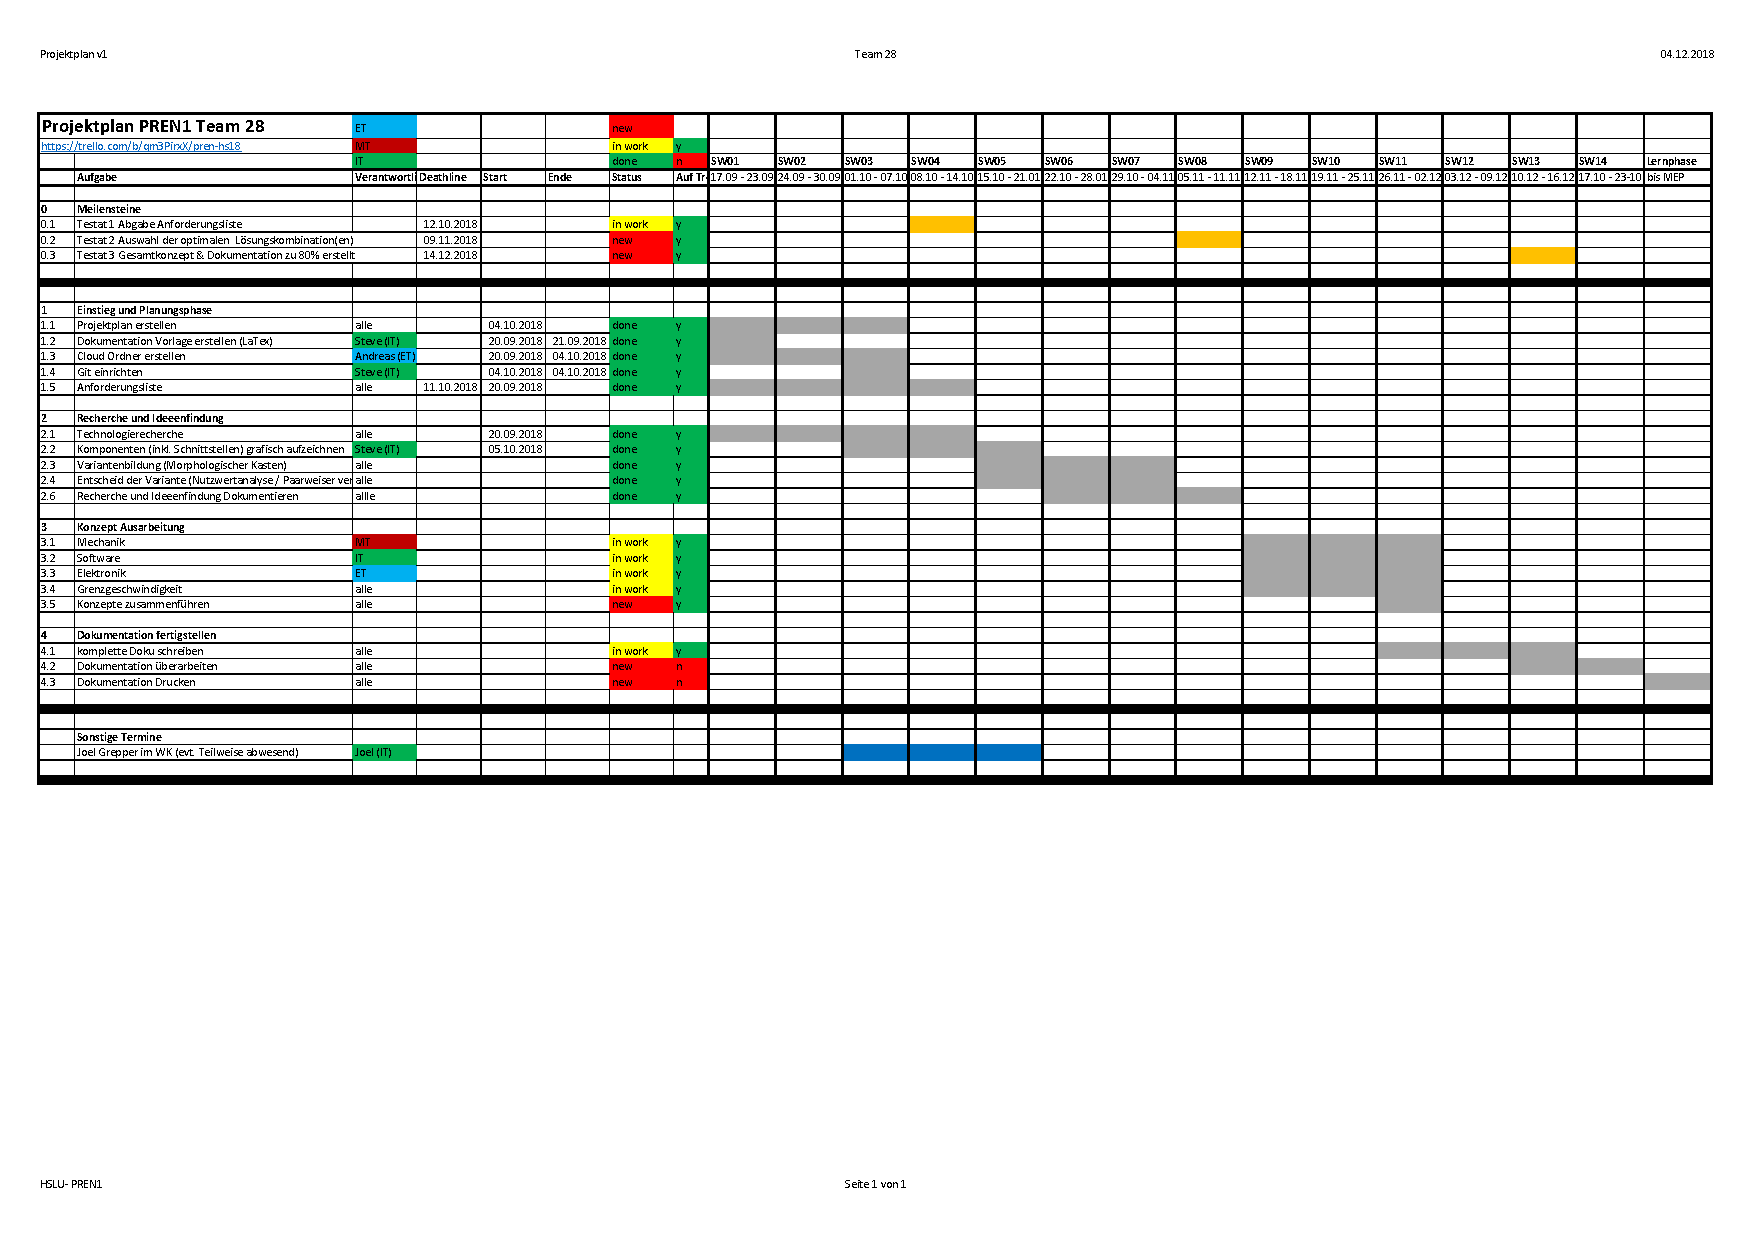
\includegraphics[page=1,width=1\textwidth, trim=.6cm 7cm .6cm 1.5cm, clip]{Projektplanung.pdf}
    \caption{Zeitorientierte Projektstruktur Team 28\\Stand: SW 12}
    \label{fig:projektplanung}
\end{figure}

Die detailliertere Aufteilung dieser Arbeitspakete wird dann in Trello (Abbliding \ref{fig:screenTrello}) vorgenommen. In der Projektstruktur wird lediglich eingetragen ob ein bestimmtes Arbeitspaket darin in Trello erfasst ist. Dort kann es in mehrere Teilpakete aufgeteilt werden und bestimmten Personen zugewiesen werden. Die Arbeitspakete in Trello werden je nach Status in die Kategorien "To do", "doing", oder "done". Separat werden auch noch die Meilensteine festgehaltne und als "done" gekennzeichnet sobald diese abgeschlossen sind.\\

\begin{figure}[H] \centering
    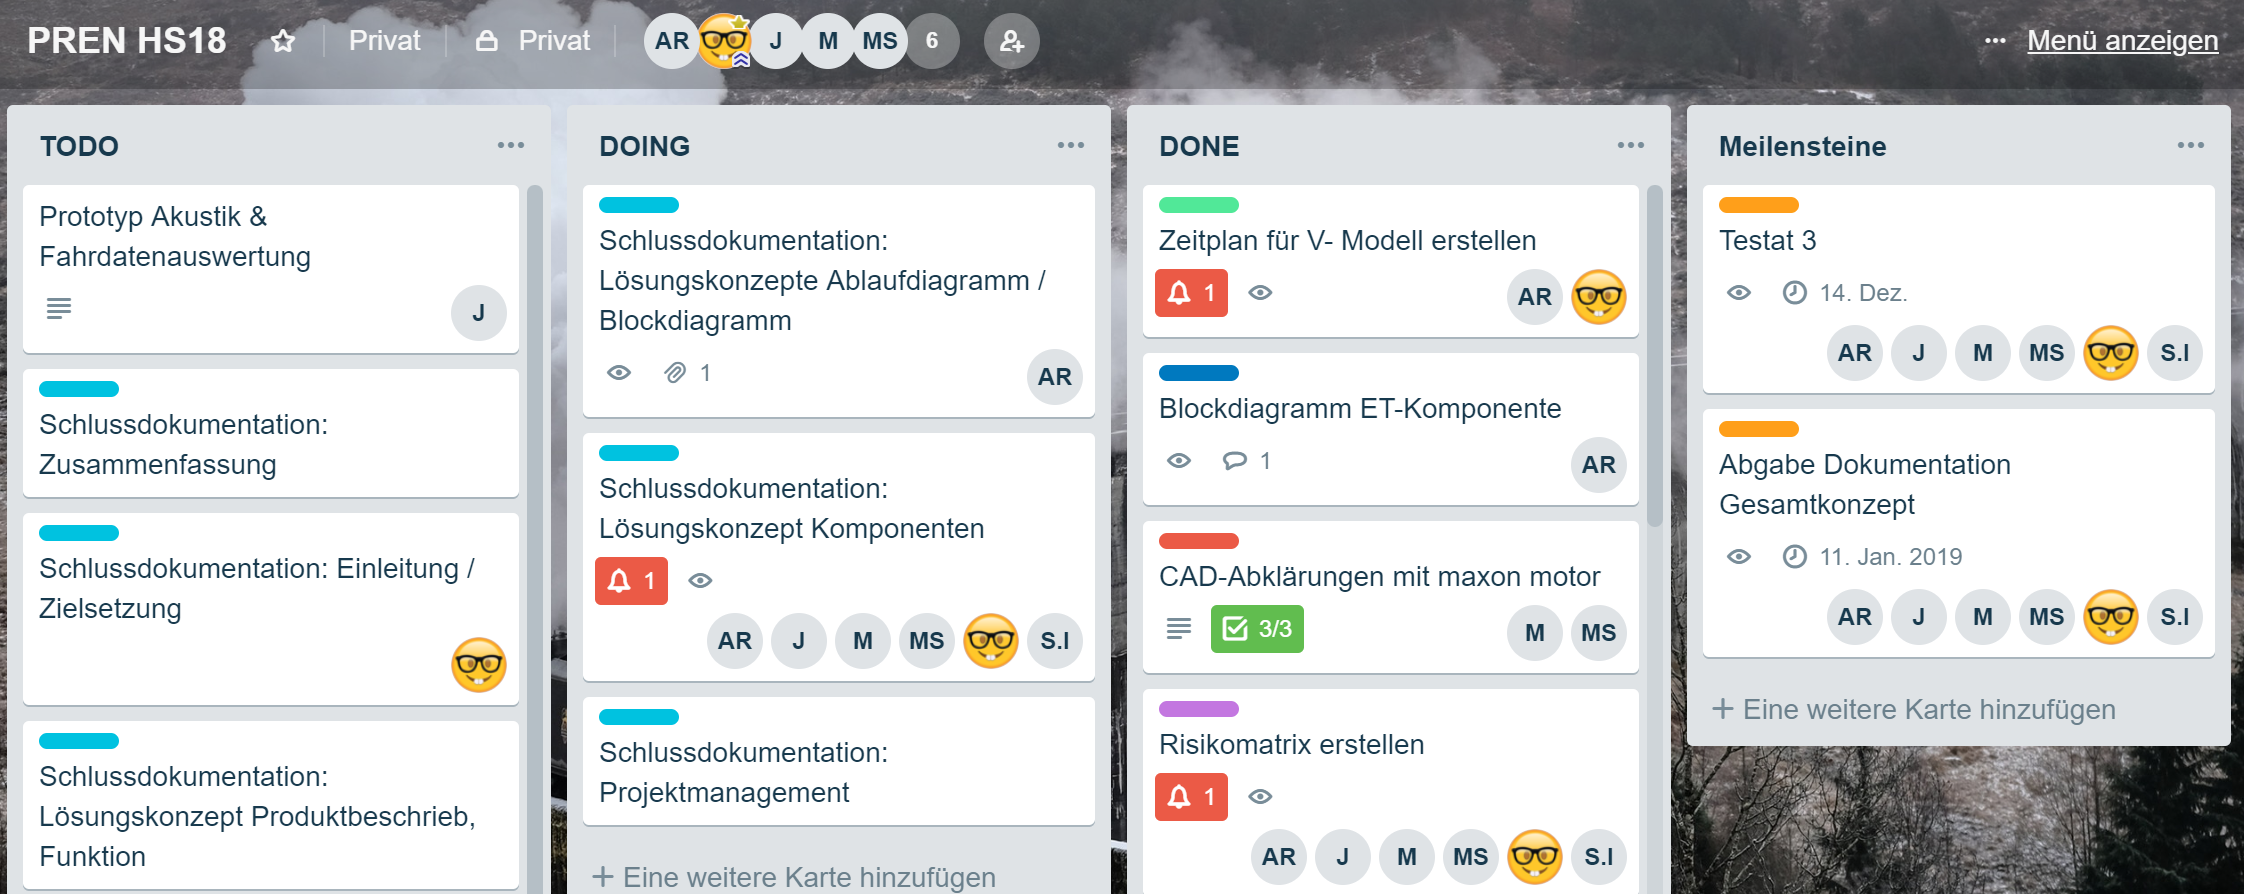
\includegraphics[page=1,width=.8\textwidth]{screenTrello.png}
    \caption{Bildschirmausschnitt Trello Team 28\\Stand: SW 12}
    \label{fig:screenTrello}
\end{figure}


\end{document}